\section{Climate Data Visualization Summary}\label{annexe:climate-viz-summary}

\subsubsection{Spatial Patterns}

Figure~\ref{fig:spatial_heatmaps} illustrates spatial heatmaps of mean climate conditions over the 2020–2024 period.

\begin{figure}[H]
    \centering
    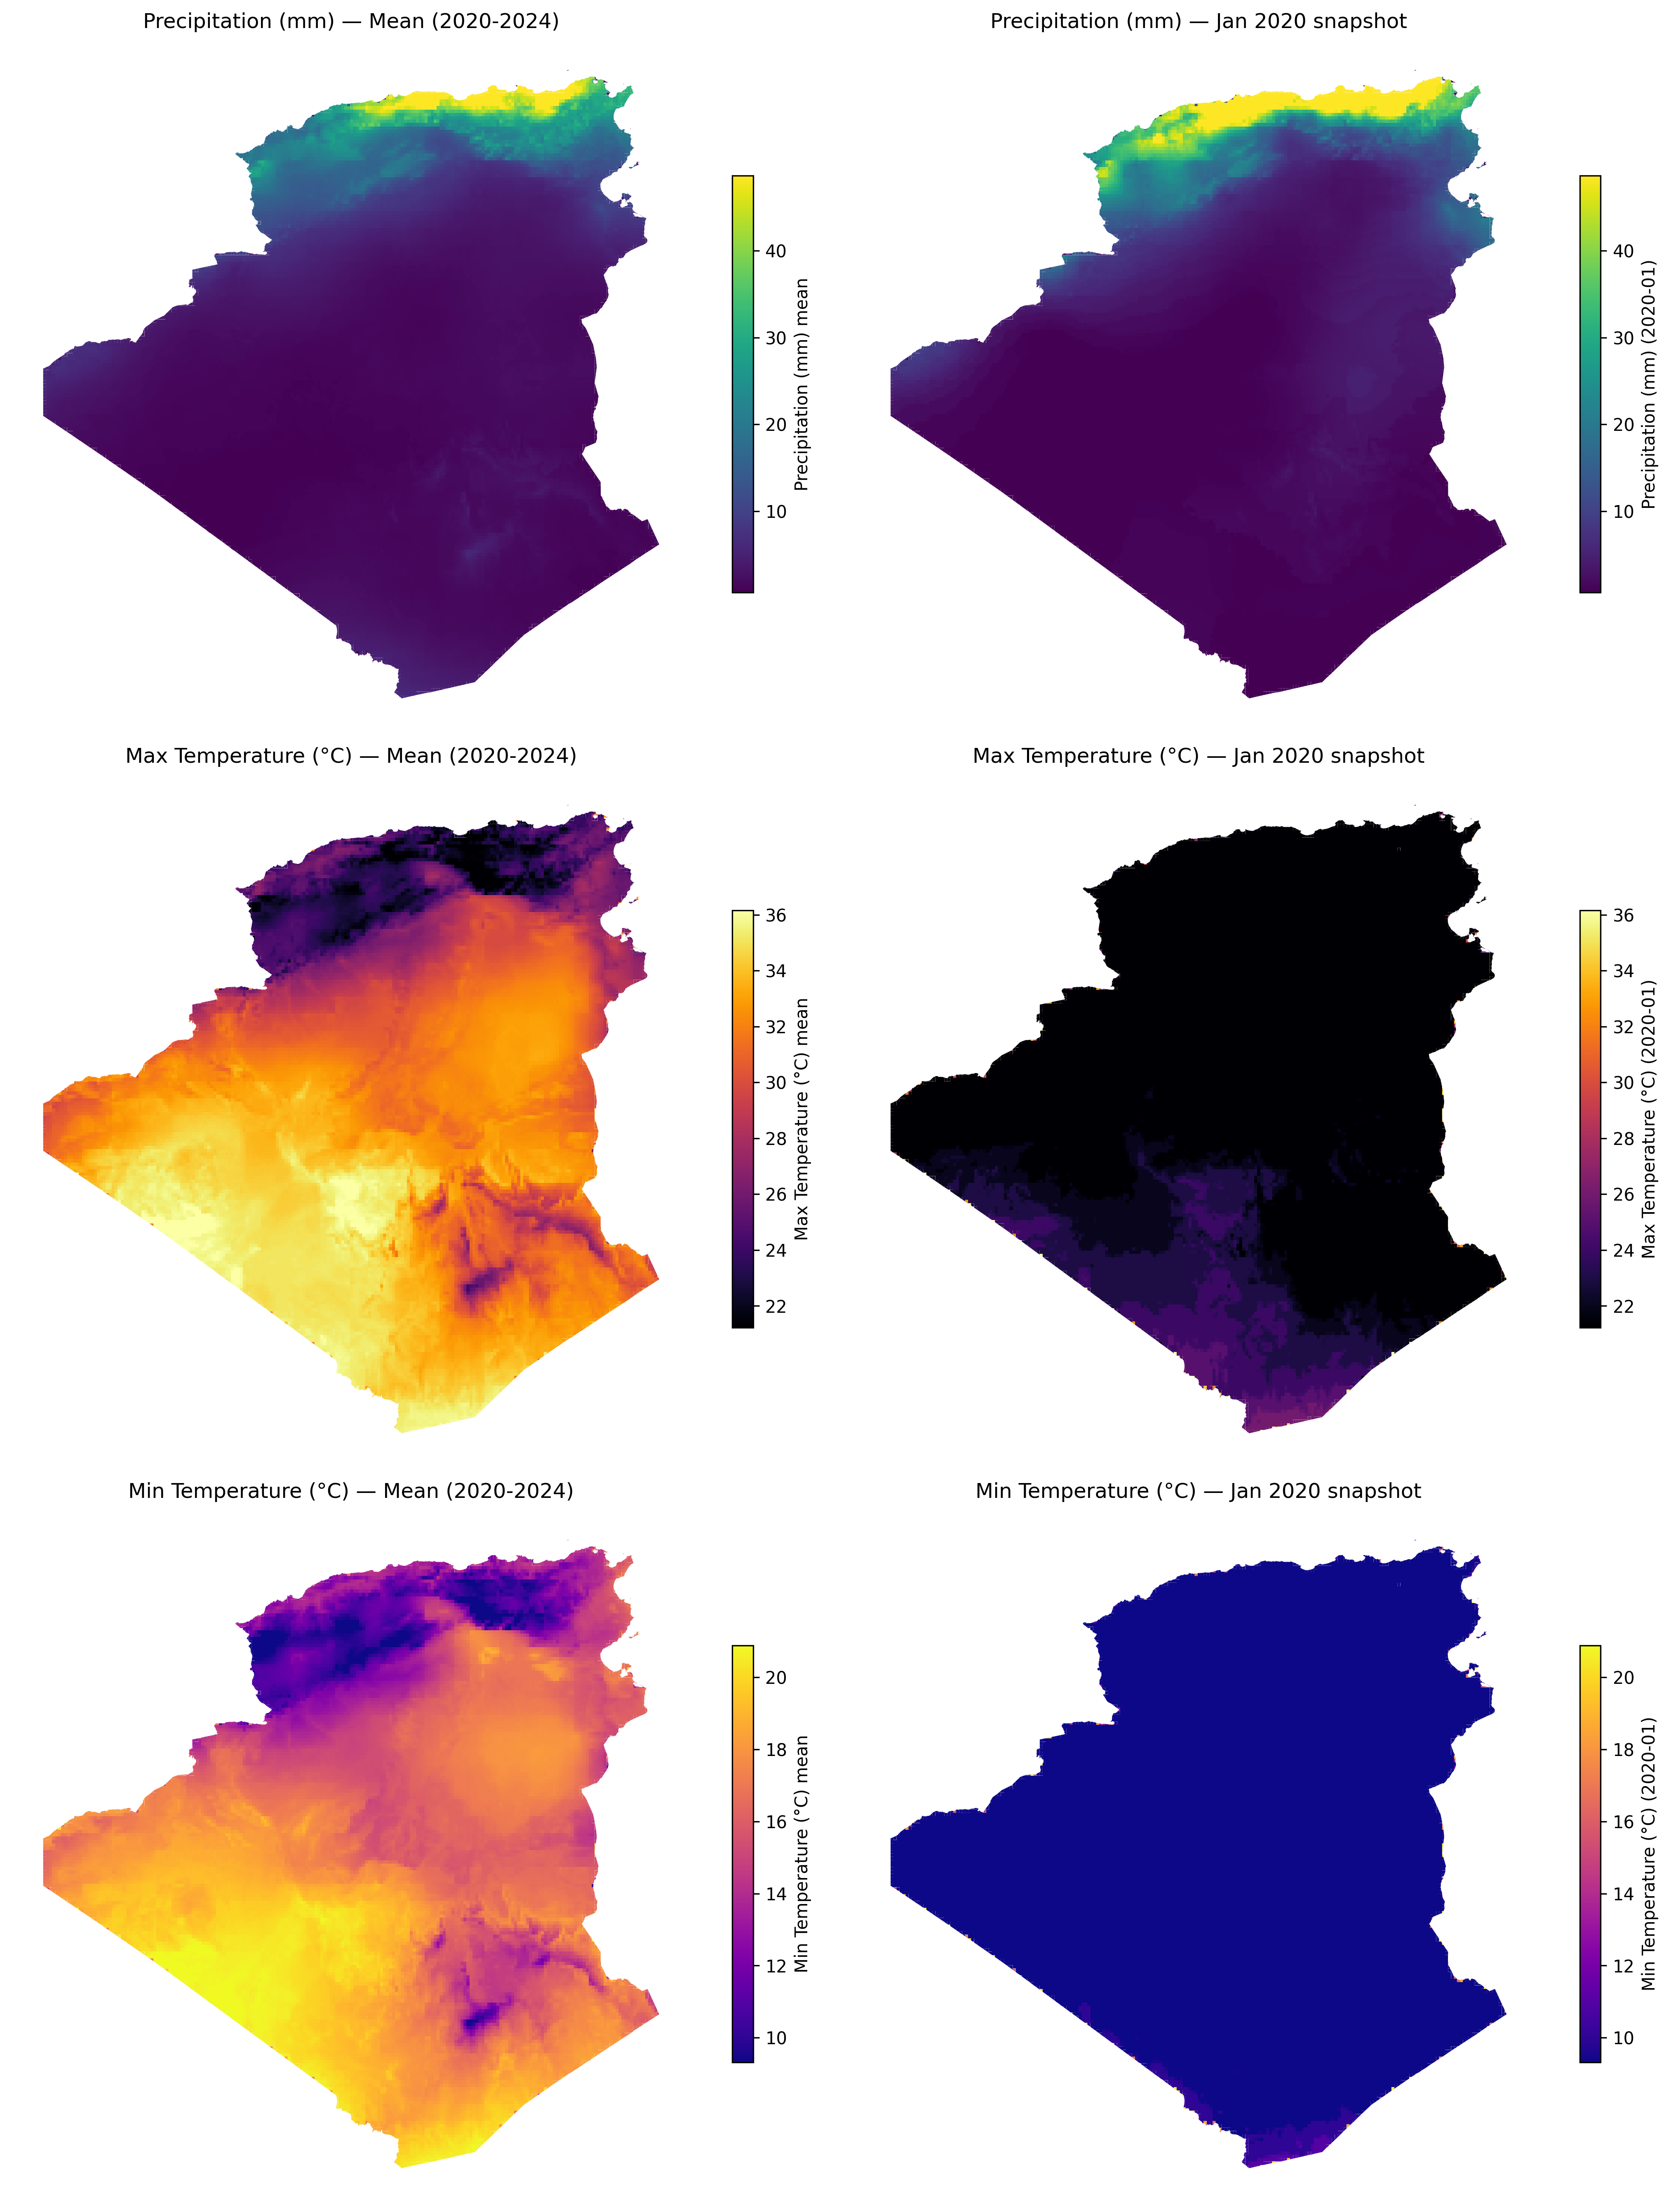
\includegraphics[width=0.5\linewidth]{images/Climate/spatial_heatmaps_all_variables.png}
    \caption{Spatial heatmaps of mean precipitation, maximum temperature, and minimum temperature (2020--2024).}
    \label{fig:spatial_heatmaps}
\end{figure}

\subsubsection{Inter-variable Relationships}

Scatter plots comparing precipitation with minimum and maximum temperatures (Figure~\ref{fig:prec_temp_scatter}) reveal moderate negative correlations ($r=-0.236$ for Tmin, $r=-0.335$ for Tmax, $p<0.001$). Higher precipitation values are associated with lower temperatures, consistent with physical processes such as cloud cover, evaporation, and seasonal rainfall regimes.

\begin{figure}[H]
    \centering
    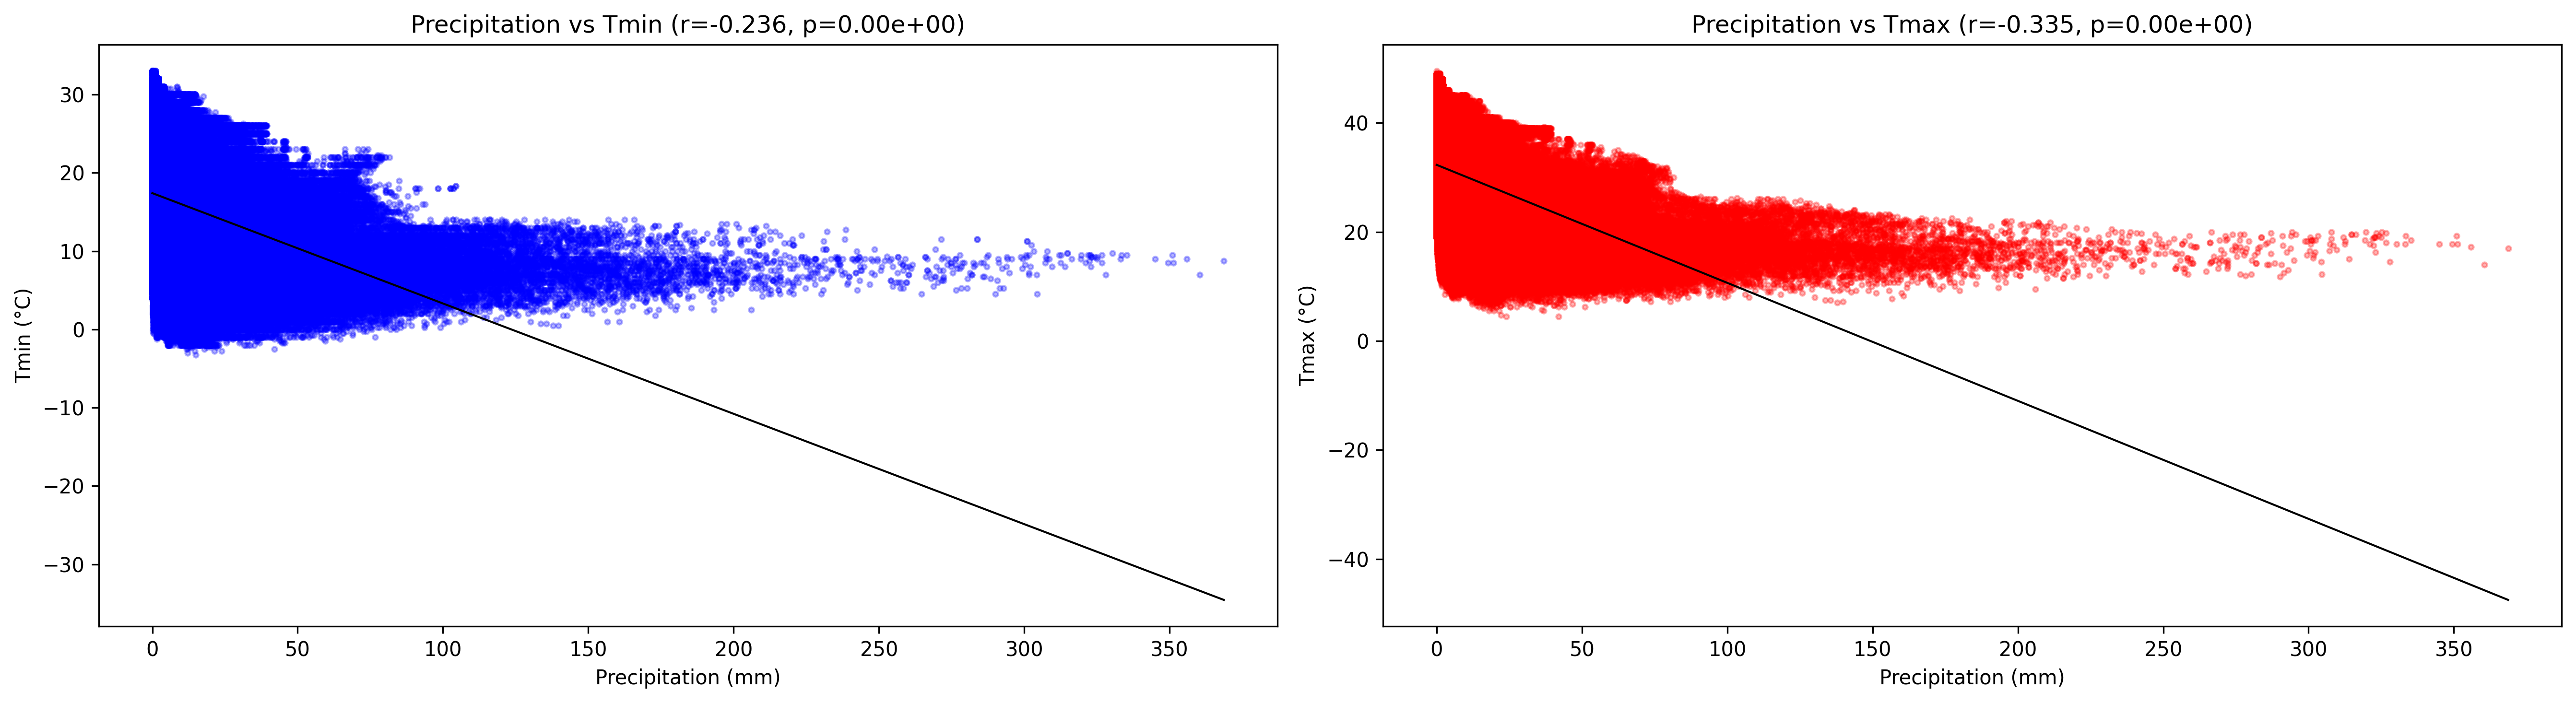
\includegraphics[width=0.95\linewidth]{images/Climate/prec_vs_temperature_scatter.png}
    \caption{Relationship between precipitation and temperature variables.}
    \label{fig:prec_temp_scatter}
\end{figure}
